\documentclass{article}
\usepackage{graphicx}
\usepackage{tikz}
\usepackage{multirow}
%\documentclass{article}
\usetikzlibrary{positioning}
\usetikzlibrary{3d} % Para trabajar con proyecciones 3D
%\usetikzlibrary{tikz-3dplot}
%\usepackage[spanish]{babel}
\usetikzlibrary{shapes.misc, arrows, positioning}
\usepackage{float}
\usepackage{amsmath}
\usepackage{tikz-3dplot}
\usepackage{pgfplots}
\usepackage{wrapfig}
\usepackage{verbatim}
\usepackage{amssymb}
\usepackage{empheq}
\usepackage{unicode-math}
\usepackage[utf8]{inputenc}
\pgfplotsset{compat=1.18}
\usepackage{capt-of}

\begin{document}


\section{Introduction}

El cálculo vectorial es una rama fundamental de las matemáticas que extiende los conceptos del cálculo diferencial e integral a funciones vectoriales, también conocidas como campos vectoriales. Su importancia radica en su amplia utilidad en diversas áreas de la ciencia y la ingeniería, especialmente en la descripción y análisis de fenómenos físicos como el electromagnetismo, la mecánica de fluidos, la elasticidad y la transferencia de calor. En ingeniería electrónica, el cálculo vectorial es esencial para comprender fenómenos como la propagación de ondas electromagnéticas en guías de onda y antenas, el comportamiento de campos en dispositivos semiconductores y el análisis de circuitos en régimen permanente sinusoidal, donde las magnitudes se representan mediante fasores (vectores en el plano complejo). También es fundamental en el estudio de sistemas de control, robótica y procesamiento de señales, donde se modelan sistemas dinámicos mediante ecuaciones diferenciales vectoriales.

En el contexto del electromagnetismo, el cálculo vectorial proporciona las herramientas necesarias para comprender y manipular las ecuaciones de Maxwell, que gobiernan el comportamiento de los campos eléctricos y magnéticos. Con estas ecuaciones vamos a culminar el análisis del electromagnetismo antes de entrar a estudiar los medios de enlace (específicamente, líneas de transmisión, guías de onda, fibras ópticas y antenas, a medida que aumenta la frecuencia o el ancho de banda). Los campos vectoriales, que asignan un vector a cada punto del espacio, son esenciales para representar magnitudes como la fuerza, la velocidad, el campo eléctrico y el campo magnético.

A lo largo de este capítulo, exploraremos los conceptos fundamentales del cálculo vectorial, que incluyen la integración y diferenciación de campos escalares y vectoriales. Como se explicó en el capítulo anterior, un \textbf{campo escalar} es una función que asigna un valor escalar (un número) a cada punto del espacio. Ejemplos comunes incluyen el potencial eléctrico, la densidad de carga y la temperatura. Por otro lado, un \textbf{campo vectorial} asigna un vector a cada punto del espacio, como se mencionó anteriormente.

Para visualizar mejor estos conceptos, consideremos algunos ejemplos cotidianos. La temperatura en una habitación se puede representar como un campo escalar, donde cada punto tiene asociado un valor de temperatura. Si abrimos una ventana en un día frío, la temperatura variará en diferentes puntos de la habitación, creando un gradiente de temperatura. Por otro lado, el flujo de aire en la misma habitación se puede representar como un campo vectorial, donde cada punto tiene asociado un vector que indica la dirección y la velocidad del aire. En este capítulo, explicaremos en detalle el concepto de gradiente y todas las operaciones que se pueden aplicar a los campos vectoriales, así como todos los elementos necesarios para definirlos correctamente.

\begin{center}
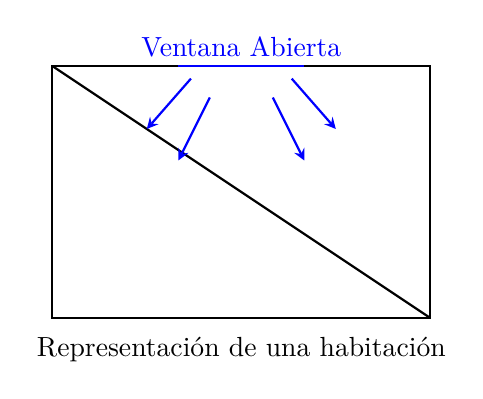
\begin{tikzpicture}[scale=0.8]
  % Habitación
  \draw[thick] (0,0) rectangle (6,4);
  \draw[thick] (0,4) -- (6,0);

  % Ventana
  \draw[thick, blue] (2,4) -- (4,4);

  % Flechas de flujo de aire (campo vectorial)
  \draw[->,>=stealth,thick,blue] (2.5,3.5) -- (2,2.5);
  \draw[->,>=stealth,thick,blue] (3.5,3.5) -- (4,2.5);
  \draw[->,>=stealth,thick,blue] (2.2,3.8) -- (1.5,3);
  \draw[->,>=stealth,thick,blue] (3.8,3.8) -- (4.5,3);

  % Etiquetas
  \node[blue] at (3,4.3) {Ventana Abierta};
  \node at (3,-0.5) {Representación de una habitación};

\end{tikzpicture}
\end{center}

La figura anterior ilustra de manera simple el concepto de un campo vectorial. La ventana abierta permite el ingreso de aire frío creando un flujo que representamos mediante vectores, simulando las partículas del aire que ingresan. \textbf{Es importante destacar que un campo vectorial, como el ilustrado, necesita expresar tanto su magnitud como su dirección en cada punto del espacio.}

El objetivo principal de este capítulo es proporcionar una base sólida en cálculo vectorial que permita comprender y resolver problemas relacionados con campos vectoriales. Comenzaremos estudiando las operaciones de integración, como las integrales de línea, superficie y volumen. Luego, nos adentraremos en las operaciones de diferenciación, como el gradiente, la divergencia y el rotacional, y exploraremos su interpretación geométrica y física. Finalmente, presentaremos algunos teoremas fundamentales, como el teorema de la divergencia, el teorema de Stokes y el teorema de Helmholtz. Este último es crucial en la teoría electromagnética, ya que permite descomponer un campo vectorial en componentes irrotacional y solenoidal. \textbf{Más adelante, estudiaremos en detalle estos conceptos (irrotacional y solenoidal) que son propiedades importantes de los campos vectoriales, como el campo eléctrico y el campo magnético}. Estos teoremas establecen relaciones importantes entre los diferentes tipos de integrales y operadores diferenciales.

Con estos fundamentos, estaremos preparados para abordar temas más avanzados en electromagnetismo y otras áreas de la ingeniería electrónica que se basan en el lenguaje del cálculo vectorial.  El formalismo matemático que estamos introduciendo aquí servirá como una base sólida para la notación compacta utilizada en electromagnetismo. Esta notación, aunque a veces puede parecer compleja para quienes no están familiarizados con ella, es una herramienta poderosa y eficiente para describir fenómenos electromagnéticos. Dominar este lenguaje matemático les permitirá abordar con mayor facilidad conceptos más avanzados en el futuro. 

\section{Integración de Campos}

En esta sección, extenderemos los conceptos de integración que aprendimos en el cálculo de una variable o análisis matemático I, correspondiente al plan de estudio de la carrera de Ingeniería Electrónica, al contexto de campos escalares y vectoriales. La integración de funciones vectoriales es una herramienta fundamental en el análisis de fenómenos físicos y tiene aplicaciones en áreas como el electromagnetismo, la mecánica de fluidos y la teoría del potencial. En esta guía, usaremos los términos "función" y "campo" indistintamente para referirnos a una asignación de un valor (escalar o vectorial) a cada punto del espacio. Aunque en matemáticas puras a veces se hace una distinción más rigurosa, en el contexto de la física y la ingeniería, esta equivalencia es común y no genera ambigüedad.

Recordemos que en el cálculo de una variable, la integral definida de una función $f(x)$ en un intervalo $[a, b]$ representa el área bajo la curva de la función entre esos límites. En el cálculo vectorial, consideraremos integrales sobre curvas, superficies y volúmenes, lo que nos permitirá calcular cantidades como el trabajo realizado por una fuerza a lo largo de una trayectoria, el flujo de un campo vectorial a través de una superficie, o la masa total contenida dentro de un volumen dado.

Comenzaremos nuestro estudio con las integrales de línea, que nos permiten integrar campos escalares y vectoriales a lo largo de una curva en el espacio.

\subsection{Integrales de Línea}

La integral de línea es una generalización de la integral definida a curvas en el espacio. Consideremos un campo vectorial $\vec{A}(x,y,z)$ definido en una región del espacio. Si tomamos dos puntos, $P_1$ y $P_2$, en esta región, podemos unirlos mediante una curva $C$, como se muestra en la Figura \ref{fig:integral_linea}.

\begin{figure}[h]
    \centering
    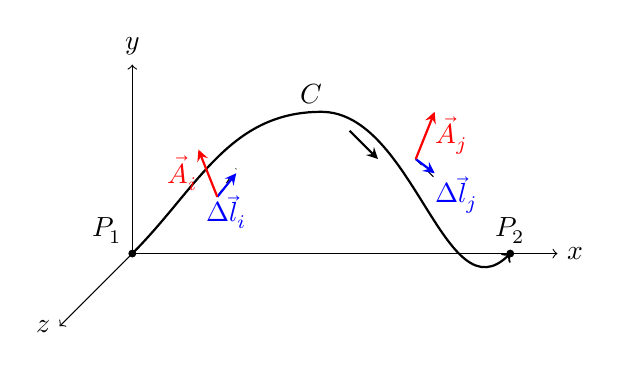
\begin{tikzpicture}[scale=1.2]
        % Dibuja la curva
        \draw[thick, ->] (0,0,0) to[out=45,in=180] (2,1.5,0) to[out=0,in=225] (4,0,0);

        % Puntos inicial y final
        \filldraw (0,0,0) circle (1pt) node[anchor=north east, above left] {$P_1$};
        \filldraw (4,0,0) circle (1pt) node[anchor=west, above] {$P_2$};

        % Etiquetas de la curva
        \node at (2, 1.8, 0.3) {$C$};

        % Flecha sobre la curva para indicar la dirección
        \draw[->, >=stealth, thick] (2.3, 1.3, 0) -- (2.6, 1, 0);

        % Segmentos
        \draw[dashed] (0.9,0.6,0) -- (1.1,0.9,0);
        \draw[dashed] (3,1,0) -- (3.2,0.8,0);

        % Vectores
        \draw[->, >=stealth, thick, blue] (0.9,0.6,0) -- (1.1,0.85,0) node[midway, below] {$\Delta \vec{l}_i$};
        \draw[->, >=stealth, thick, blue] (3,1,0) -- (3.2,0.85,0) node[midway, below right] {$\Delta \vec{l}_j$};

         % Campos vectoriales
        \draw[->, >=stealth, thick, red] (0.9,0.6,0) -- (0.7,1.1,0) node[midway, left] {$\vec{A}_i$};
        \draw[->, >=stealth, thick, red] (3,1,0) -- (3.2,1.5,0) node[midway, right] {$\vec{A}_j$};

        % Ejes
        \draw[->] (0,0,0) -- (4.5,0,0) node[right] {$x$};
        \draw[->] (0,0,0) -- (0,2,0) node[above] {$y$};
        \draw[->] (0,0,0) -- (0,0,2) node[left] {$z$};
    \end{tikzpicture}
    \caption{Integral de línea a lo largo de una curva C}
    \label{fig:integral_linea}
\end{figure}

Ahora, dividamos la curva $C$ en $n$ segmentos pequeños de longitud $\Delta l_i$, donde $i = 1, 2, ..., n$. En cada segmento, podemos definir un vector $\Delta \vec{l}_i$ que tenga la magnitud $\Delta l_i$ y la dirección tangente a la curva en ese segmento, en el sentido de $P_1$ a $P_2$.

Podemos aproximar la proyección del campo vectorial $\vec{A}$ sobre cada segmento $\Delta \vec{l}_i$ mediante el producto escalar $\vec{A_i} \cdot \Delta \vec{l}_i$, donde $\vec{A_i}$ es el valor del campo vectorial en algún punto del segmento $i$. Si ahora sumamos estas proyecciones a lo largo de la curva $C$, obtenemos una aproximación de la integral de línea de $\vec{A}$ a lo largo de $C$:

\[
\sum_{i=1}^n \vec{A}_i \cdot \Delta \vec{l}_i
\]

Para obtener la integral de línea exacta, tomamos el límite cuando la longitud de los segmentos tiende a cero (es decir, cuando $n$ tiende a infinito y $\Delta l_i$ tiende a cero). En este límite, la suma se convierte en una integral, y el elemento de longitud $\Delta \vec{l}_i$ se convierte en el diferencial de longitud de arco $d\vec{l}$:

\[
\int_C \vec{A} \cdot d\vec{l} = \lim_{n \to \infty, \Delta l_i \to 0} \sum_{i=1}^n \vec{A}_i \cdot \Delta \vec{l}_i
\]

Esta relación, que se muestra en la ecuación enmarcada a continuación, es fundamental para comprender el significado físico de la integral de línea de un campo vectorial:

\begin{equation}
\boxed{\int_C \vec{A} \cdot d\vec{l} = \int_C |\vec{A}| \, |d\vec{l}| \, \cos \theta}
\label{eq:int_linea_destacada}
\end{equation}

\textbf{Interpretación: La integral de línea de un campo vectorial $\vec{A}$ a lo largo de una curva $C$ representa la suma de las proyecciones del campo sobre la tangente a la curva en cada punto, a lo largo de toda la curva. Es decir, la integral de línea cuantifica la componente del campo vectorial que es paralela a la curva en cada punto. Donde, $\theta$ es el ángulo formado entre el vector del campo $\vec{A}$ y el vector tangente a la curva $d\vec{l}$.}

\subsubsection{Circulación de un campo vectorial}

Cuando la curva $C$ es cerrada, es decir, cuando el punto final $P_2$ coincide con el punto inicial $P_1$, la integral de línea se denomina \textbf{circulación} (o integral de línea cerrada) del campo vectorial $\vec{A}$ alrededor de $C$. La circulación se denota con un símbolo de integral con un círculo superpuesto:

\begin{equation}
\oint_C \vec{A} \cdot d\vec{l}
\end{equation}

La circulación mide la tendencia del campo vectorial a "girar" alrededor de la curva cerrada. Intuitivamente, si imaginamos el campo vectorial como un fluido en movimiento, la circulación nos indica si el fluido tiende a girar en remolinos alrededor de la curva cerrada.

\subsubsection{Campos conservativos y no conservativos}

La circulación es un concepto clave para distinguir entre campos vectoriales conservativos y no conservativos.

\textbf{Campo conservativo:} Un campo vectorial $\vec{A}$ se denomina \textbf{conservativo} si la integral de línea entre dos puntos cualesquiera es independiente de la trayectoria seguida y, por lo tanto, la circulación alrededor de cualquier curva cerrada es cero:

\begin{equation}
\oint_C \vec{A} \cdot d\vec{l} = 0
\end{equation}

En un campo conservativo, el trabajo realizado para mover una partícula de un punto a otro solo depende de las posiciones inicial y final, y no del camino recorrido. Un ejemplo de campo conservativo es el campo electrostático. Como veremos en el siguiente capítulo, este campo tiene la propiedad de que su circulación alrededor de cualquier curva cerrada es siempre cero.

\textbf{Campo no conservativo:} Un campo vectorial $\vec{A}$ se denomina \textbf{no conservativo} si la integral de línea entre dos puntos depende de la trayectoria seguida. En consecuencia, la circulación alrededor de una curva cerrada puede ser distinta de cero:

\begin{equation}
\oint_C \vec{A} \cdot d\vec{l} \neq 0
\end{equation}

En un campo no conservativo, el trabajo realizado para mover una partícula de un punto a otro depende del camino recorrido. Un ejemplo de campo no conservativo es el campo magnético inducido por una corriente variable. En este caso, la circulación alrededor de una curva cerrada puede ser distinta de cero, dependiendo de la variación de la corriente que induce el campo.

Si en lugar de un campo vectorial tenemos un campo escalar $f(x,y,z)$, la integral de línea se define de manera similar, pero en lugar del producto escalar, simplemente multiplicamos el valor del campo escalar por la longitud del elemento de arco:

\[
\int_C f(x, y, z) \, dl = \lim_{n \to \infty, \Delta l_i \to 0} \sum_{i=1}^n f_i \, \Delta l_i
\]

donde $f_i$ es el valor del campo escalar en algún punto del segmento $i$ y $dl$ es la magnitud del diferencial de longitud de arco a lo largo de la curva.

\subsubsection{Parametrización de una curva}

Hasta ahora, hemos definido la integral de línea de manera intuitiva, considerando una suma de proyecciones de un campo vectorial sobre segmentos a lo largo de una curva $C$. Sin embargo, para calcular efectivamente estas integrales, necesitamos una forma de describir la curva matemáticamente. Aquí es donde entra en juego la \textbf{parametrización} de la curva.\\

\textbf{¿Por qué parametrizar?}

Podríamos preguntarnos por qué introducir la parametrización, que puede parecer un paso adicional y más abstracto al principio. La respuesta radica en las ventajas que ofrece este enfoque:

\begin{itemize}
    \item \textbf{Generalidad:} La parametrización es una técnica \textbf{general} que funciona para \textbf{cualquier} tipo de curva, no solo para aquellas que se pueden expresar fácilmente en coordenadas cartesianas (x, y, z). En el estudio de electromagnetismo, es frecuente encontrarnos con curvas complejas, como hélices o espirales, para las cuales la parametrización es esencial.
    \item \textbf{Simplicidad:} Aunque la parametrización puede parecer más compleja al principio, a menudo \textbf{simplifica} el cálculo de las integrales de línea. Al parametrizar, expresamos la curva en términos de una sola variable independiente (el parámetro $t$), lo que nos permite transformar la integral de línea en una integral definida ordinaria de una sola variable, que ya sabemos cómo resolver.
    \item \textbf{Comprensión conceptual:} La parametrización ayuda a comprender mejor la naturaleza de la integral de línea como una integral \textbf{a lo largo de una curva} en el espacio, y no como una simple suma de integrales en cada coordenada (x, y, z). Nos permite "recorrer" la curva de manera continua a medida que el parámetro varía.
    \item \textbf{Conexión con la física:} En muchas aplicaciones físicas,la parametrización surge de forma natural. Por ejemplo, al calcular el trabajo realizado por una fuerza a lo largo de una trayectoria curva, la posición de la partícula a menudo se describe en función del tiempo, que actúa como parámetro natural de la curva.
\end{itemize}

En resumen, la parametrización es una técnica poderosa y general que simplifica el cálculo de integrales de línea en la mayoría de los casos. Si bien es posible resolver algunas integrales de línea simples en coordenadas cartesianas, la parametrización es el método preferido y el que prepara mejor al alumno para situaciones más complejas que sin duda surgirán en el estudio del electromagnetismo y otras áreas de la ingeniería.

Ahora, veamos cómo parametrizar una curva en el espacio. Una curva $C$ en el espacio tridimensional se puede parametrizar mediante un vector de posición $\vec{r}(t) = x(t)\hat{x} + y(t)\hat{y} + z(t)\hat{z}$, donde $t$ es un parámetro que varía en un intervalo $[a, b]$. A medida que $t$ varía de $a$ a $b$, el vector $\vec{r}(t)$ traza la curva $C$ en el espacio.

Ahora, veamos cómo parametrizar una curva en el espacio. Una curva $C$ en el espacio tridimensional se puede parametrizar mediante un vector de posición $\vec{r}(t) = x(t)\hat{x} + y(t)\hat{y} + z(t)\hat{z}$, donde $t$ es un parámetro que varía en un intervalo $[a, b]$. A medida que $t$ varía de $a$ a $b$, el vector $\vec{r}(t)$ traza la curva $C$ en el espacio.

El vector tangente a la curva en un punto dado se obtiene derivando el vector de posición con respecto al parámetro $t$:

\[
\vec{r}'(t) = \frac{d\vec{r}}{dt} = \frac{dx}{dt}\hat{x} + \frac{dy}{dt}\hat{y} + \frac{dz}{dt}\hat{z}
\]

Este vector $\vec{r}'(t)$ nos da la dirección de la tangente a la curva en el punto correspondiente al valor de $t$. La magnitud de este vector, $|\vec{r}'(t)|$, nos da la "velocidad" a la que se recorre la curva con respecto al parámetro $t$.

Recordemos que en la definición de la integral de línea, teníamos el elemento de longitud de arco $d\vec{l}$ (para el caso de un campo vectorial) y su magnitud $dl$ (para el caso de un campo escalar). Podemos expresar estos elementos en términos del parámetro $t$ y el vector tangente $\vec{r}'(t)$.

Para el caso de un campo vectorial, el elemento de longitud de arco $d\vec{l}$ se expresa como:

\[
d\vec{l} = \vec{r}'(t) \, dt = \left(\frac{dx}{dt}\hat{x} + \frac{dy}{dt}\hat{y} + \frac{dz}{dt}\hat{z}\right) dt
\]

Y para el caso de un campo escalar, la magnitud del elemento de longitud de arco $dl$ se expresa como:

\[
dl = |d\vec{l}| = |\vec{r}'(t)| \, dt = \sqrt{\left(\frac{dx}{dt}\right)^2 + \left(\frac{dy}{dt}\right)^2 + \left(\frac{dz}{dt}\right)^2} \, dt
\]

Ahora podemos expresar las integrales de línea de un campo vectorial $\vec{A}$ y un campo escalar $f$ en términos del parámetro $t$:

\textbf{Para un campo vectorial:}

\[
\int_C \vec{A} \cdot d\vec{l} = \int_a^b \vec{A}(\vec{r}(t)) \cdot \vec{r}'(t) \, dt
\]

donde $\vec{A}(\vec{r}(t))$ significa que el campo vectorial $\vec{A}$ se evalúa en los puntos de la curva parametrizada por $\vec{r}(t)$.

\textbf{Para un campo escalar:}

\[
\int_C f \, dl = \int_a^b f(\vec{r}(t)) \, |\vec{r}'(t)| \, dt
\]

donde $f(\vec{r}(t))$ significa que el campo escalar $f$ se evalúa en los puntos de la curva parametrizada por $\vec{r}(t)$.

Con estas expresiones, hemos transformado las integrales de línea a lo largo de la curva $C$ en integrales definidas ordinarias con respecto al parámetro $t$, que varían en el intervalo $[a, b]$. Esto nos permite calcular las integrales de línea utilizando las técnicas que ya conocemos del cálculo de una variable.

**Ejemplo 1 (Campo Escalar):**
Supongamos que tenemos un alambre delgado en forma de semicírculo con radio $R$ parametrizado por $\vec{r}(t) = R\cos(t)\hat{x} + R\sin(t)\hat{y}$, con $0 \le t \le \pi$. La densidad lineal de carga del alambre (carga por unidad de longitud) está dada por el campo escalar $\lambda(x, y) = \lambda_0 (1 + x/R)$, donde $\lambda_0$ es una constante. Queremos encontrar la carga total $Q$ del alambre.

**Solución:**

La carga total se puede encontrar integrando la densidad lineal de carga a lo largo de la curva. Usando la parametrización $\vec{r}(t)$, la integral de línea se convierte en:

\[
Q = \int_C \lambda(x, y) \, dl = \int_0^{\pi} \lambda(\vec{r}(t)) |\vec{r}'(t)| \, dt
\]

donde $\lambda(\vec{r}(t))$ significa que evaluamos el campo escalar $\lambda(x,y)$ en las coordenadas parametrizadas $(x(t), y(t)) = (R\cos(t), R\sin(t))$.

**1. Calculamos $\vec{r}'(t)$:**

\[
\vec{r}'(t) = \frac{d\vec{r}}{dt} = -R\sin(t)\hat{x} + R\cos(t)\hat{y}
\]

**2. Calculamos $|\vec{r}'(t)|$:**

\[
|\vec{r}'(t)| = \sqrt{(-R\sin(t))^2 + (R\cos(t))^2} = \sqrt{R^2(\sin^2(t) + \cos^2(t))} = R
\]

**3. Evaluamos $\lambda(\vec{r}(t))$:**

\[
\lambda(\vec{r}(t)) = \lambda(R\cos(t), R\sin(t)) = \lambda_0 \left(1 + \frac{R\cos(t)}{R}\right) = \lambda_0 (1 + \cos(t))
\]

**4. Sustituimos en la integral:**

\[
Q = \int_0^{\pi} \lambda_0 (1 + \cos(t)) \, R \, dt = \lambda_0 R \int_0^{\pi} (1 + \cos(t)) \, dt
\]

**5. Resolvemos la integral:**

\[
Q = \lambda_0 R [t + \sin(t)]_0^{\pi} = \lambda_0 R [(\pi + \sin(\pi)) - (0 + \sin(0))] = \lambda_0 R \pi
\]

Por lo tanto, la carga total del alambre es $Q = \lambda_0 R \pi$.

\begin{center}
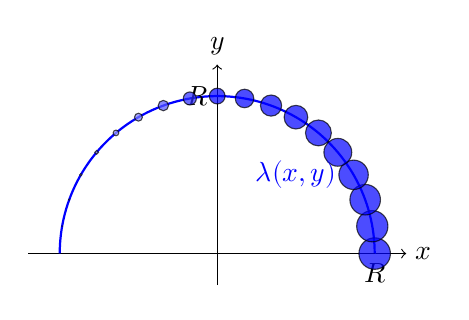
\begin{tikzpicture}[scale=2]
    % Ejes
    \draw[->] (-1.2,0) -- (1.2,0) node[right] {$x$};
    \draw[->] (0,-0.2) -- (0,1.2) node[above] {$y$};

    % Semicircunferencia
    \draw[domain=0:pi,samples=100,thick,blue] plot ({cos(\x r)}, {sin(\x r)});

    % Etiquetas de los ejes
    \node[below] at (1,0) {$R$};
    \node[left] at (0,1) {$R$};

    % Radio
    \draw[dashed] (0,0) -- (1,0);

    % Densidad de carga (representación visual)
    \foreach \x in {0,10,...,180} {
        \pgfmathsetmacro{\densidad}{1 + cos(\x)}; % Calcula la densidad
        \pgfmathsetmacro{\densidadcien}{\densidad*100}; % Multiplica por 100
        \pgfmathsetmacro{\radio}{0.05*\densidad}; % Ajusta el radio del círculo
        \draw[fill=blue!\densidadcien, opacity=0.7] ({cos(\x)}, {sin(\x)}) circle ({\radio}); % Dibuja un círculo con color y radio variables
    }

    % Etiqueta de la densidad de carga
    \node[blue] at (0.5,0.5) {$\lambda(x,y)$};
\end{tikzpicture}
\end{center}

La figura anterior muestra la representación del alambre semicircular. La variación en el color y el tamaño de los círculos a lo largo del alambre representa la densidad lineal de carga $\lambda(x, y)$, que es mayor en el lado derecho ($x > 0$) y menor en el lado izquierdo ($x < 0$).

\textbf{Ejemplo (Parametrización de una hélice):}

Consideremos una hélice circular de radio $R$, paso $p$ (distancia entre dos vueltas consecutivas) y que se extiende a lo largo del eje $z$. Podemos parametrizar esta hélice mediante el vector de posición:

\[
\vec{r}(t) = R\cos(t)\hat{x} + R\sin(t)\hat{y} + \frac{pt}{2\pi}\hat{z}
\]

donde $t$ es el parámetro que varía a lo largo de la hélice. Un valor de $t = 0$ corresponde al inicio de la hélice, y cada aumento de $2\pi$ en $t$ corresponde a una vuelta completa alrededor del eje $z$.

Calculemos la integral de línea del campo vectorial $\vec{F}(x, y, z) = -y\hat{x} + x\hat{y} + z\hat{z}$ a lo largo de una vuelta completa de la hélice.

1. Derivada del vector de posición:

\[
\vec{r}'(t) = \frac{d\vec{r}}{dt} = -R\sin(t)\hat{x} + R\cos(t)\hat{y} + \frac{p}{2\pi}\hat{z}
\]

2. Magnitud de la derivada:

\[
|\vec{r}'(t)| = \sqrt{(-R\sin(t))^2 + (R\cos(t))^2 + \left(\frac{p}{2\pi}\right)^2} = \sqrt{R^2 + \left(\frac{p}{2\pi}\right)^2}
\]

3. Evaluación del campo vectorial en la curva:

\[
\vec{F}(\vec{r}(t)) = \vec{F}(R\cos(t), R\sin(t), \frac{pt}{2\pi}) = -R\sin(t)\hat{x} + R\cos(t)\hat{y} + \frac{pt}{2\pi}\hat{z}
\]

4. Producto punto:

\[
\vec{F}(\vec{r}(t)) \cdot \vec{r}'(t) = (-R\sin(t))(-R\sin(t)) + (R\cos(t))(R\cos(t)) + \left(\frac{pt}{2\pi}\right)\left(\frac{p}{2\pi}\right) = R^2 + \frac{p^2t}{(2\pi)^2}
\]

5. Integral de línea:

Para una vuelta completa de la hélice, $t$ varía de $0$ a $2\pi$. Entonces, la integral de línea es:

\[
\int_C \vec{F} \cdot d\vec{l} = \int_0^{2\pi} \vec{F}(\vec{r}(t)) \cdot \vec{r}'(t) \, dt = \int_0^{2\pi} \left(R^2 + \frac{p^2t}{(2\pi)^2}\right) dt
\]

\[
= \left[R^2t + \frac{p^2t^2}{2(2\pi)^2}\right]_0^{2\pi} = 2\pi R^2 + \frac{p^2(2\pi)^2}{2(2\pi)^2} = 2\pi R^2 + \frac{p^2}{2}
\]

Resultado:

La integral de línea del campo vectorial $\vec{F}$ a lo largo de una vuelta completa de la hélice es $2\pi R^2 + \frac{p^2}{2}$.

\begin{center}
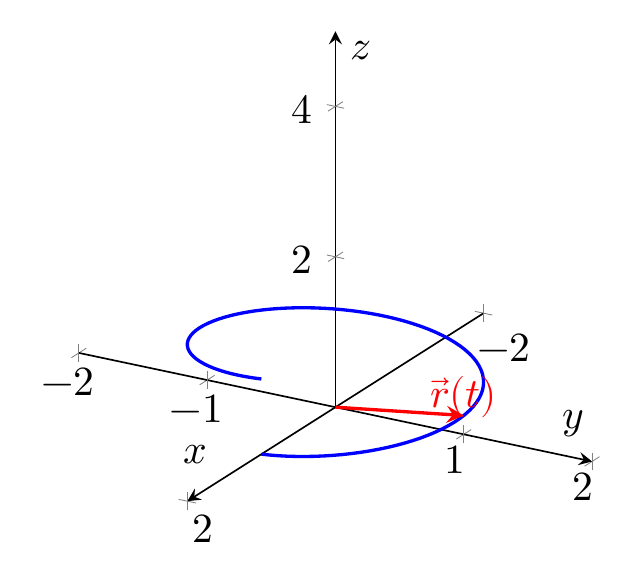
\begin{tikzpicture}[scale=1.5]
    \begin{axis}[
        axis lines=center,
        xlabel={$x$}, ylabel={$y$}, zlabel={$z$},
        xmin=-2, xmax=2,
        ymin=-2, ymax=2,
        zmin=0, zmax=5,
        view={120}{30}
    ]

    % Hélice
    \addplot3[domain=0:2*pi, samples=100, thick, blue, samples y=0] ({cos(deg(x))}, {sin(deg(x))}, {x/(2*pi)});

    % Vector de posición (ejemplo en t=pi/2)
    \addplot3[->, >=stealth, thick, red] coordinates {(0,0,0) (0,1,0.25)};
    \node[red] at (axis cs:0,1,0.5) {$\vec{r}(t)$};

    \end{axis}
\end{tikzpicture}
\end{center}

La figura anterior muestra la gráfica de una hélice circular con radio $R=1$ y paso $p=1$. El vector rojo representa el vector de posición $\vec{r}(t)$ para un valor particular de $t$ (en este caso, $t=\pi/2$).


\textbf{Ejemplo 2 (Campo Vectorial):}
Calcular la diferencia de potencial eléctrico entre dos puntos $A$ y $B$ en un campo eléctrico no uniforme dado por $\vec{E}(x, y, z) = 2x\hat{x} - 4y\hat{y} + \hat{z}$ a lo largo de una trayectoria recta desde $A = (0, 0, 0)$ hasta $B = (1, 1, 1)$.

La diferencia de potencial eléctrico $V_B - V_A$ se calcula como la integral de línea del campo eléctrico a lo largo de la trayectoria:

\[
V_B - V_A = -\int_A^B \vec{E} \cdot d\vec{r}
\]

Parametrizamos la trayectoria recta desde $A$ hasta $B$ como $\vec{r}(t) = t\hat{x} + t\hat{y} + t\hat{z}$, donde $0 \le t \le 1$. Entonces, $\vec{r}'(t) = \hat{x} + \hat{y} + \hat{z}$.

Evaluamos $\vec{E}$ en términos de $t$:

\[
\vec{E}(\vec{r}(t)) = 2t\hat{x} - 4t\hat{y} + \hat{z}
\]

Calculamos el producto punto:

\[
\vec{E}(\vec{r}(t)) \cdot \vec{r}'(t) = (2t)(1) + (-4t)(1) + (1)(1) = 2t - 4t + 1 = 1 - 2t
\]

Finalmente, integramos con respecto a $t$:

\[
V_B - V_A = -\int_0^1 (1 - 2t) \ dt = -[t - t^2]_0^1 = -(1 - 1) = 0
\]

Por lo tanto, la diferencia de potencial eléctrico entre los puntos $A$ y $B$ a lo largo de la trayectoria especificada es 0. Esto indica que el trabajo realizado por el campo eléctrico para mover una carga de prueba a lo largo de esta trayectoria es cero.

\begin{center}
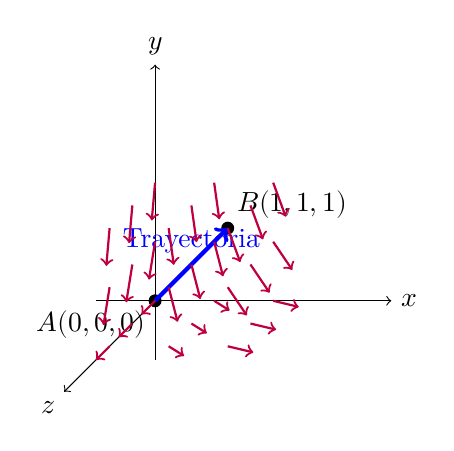
\begin{tikzpicture}[scale=1.5]
    % Ejes
    \draw[->] (-0.5,0,0) -- (2,0,0) node[right] {$x$};
    \draw[->] (0,-0.5,0) -- (0,2,0) node[above] {$y$};
    \draw[->] (0,0,-0.5) -- (0,0,2) node[anchor=north east] {$z$};

    % Puntos A y B
    \filldraw[black] (0,0,0) circle (0.05) node[anchor=north east] {$A(0,0,0)$};
    \filldraw[black] (1,1,1) circle (0.05) node[anchor=south west] {$B(1,1,1)$};

    % Trayectoria (línea recta de A a B)
    \draw[thick, blue, ->, line width=1.5pt] (0,0,0) -- (1,1,1) node[midway, above] {Trayectoria};

    % Campo eléctrico (rejilla de vectores - MENOS DENSA)
    \foreach \x in {0,0.5,1} { % Se reduce la densidad en x
        \foreach \y in {0,0.5,1} { % Se reduce la densidad en y
            \foreach \z in {0,0.5,1} { % Se reduce la densidad en z
                \pgfmathsetmacro{\u}{2*\x};
                \pgfmathsetmacro{\v}{-4*\y};
                \pgfmathsetmacro{\w}{1};
                \pgfmathsetmacro{\norm}{sqrt((\u)^2+(\v)^2+(\w)^2)};
                \pgfmathsetmacro{\scale}{0.3}; % Factor de escala para los vectores (ajustado)

                % Dibuja el vector (normalizado)
                \draw[->, purple, thick] (\x,\y,\z) -- ++({\scale*\u/\norm},{\scale*\v/\norm},{\scale*\w/\norm});
            }
        }
    }
\end{tikzpicture}
\end{center}


Finalmente, integramos con respecto a $t$:

\[
V_B - V_A = -\int_0^1 (1 - 2t) \ dt = -[t - t^2]_0^1 = -(1 - 1) = 0
\]

Por lo tanto, la diferencia de potencial eléctrico entre los puntos $A$ y $B$ a lo largo de la trayectoria especificada es 0. Esto indica que el trabajo realizado por el campo eléctrico para mover una carga de prueba a lo largo de esta trayectoria es cero.

\begin{center}
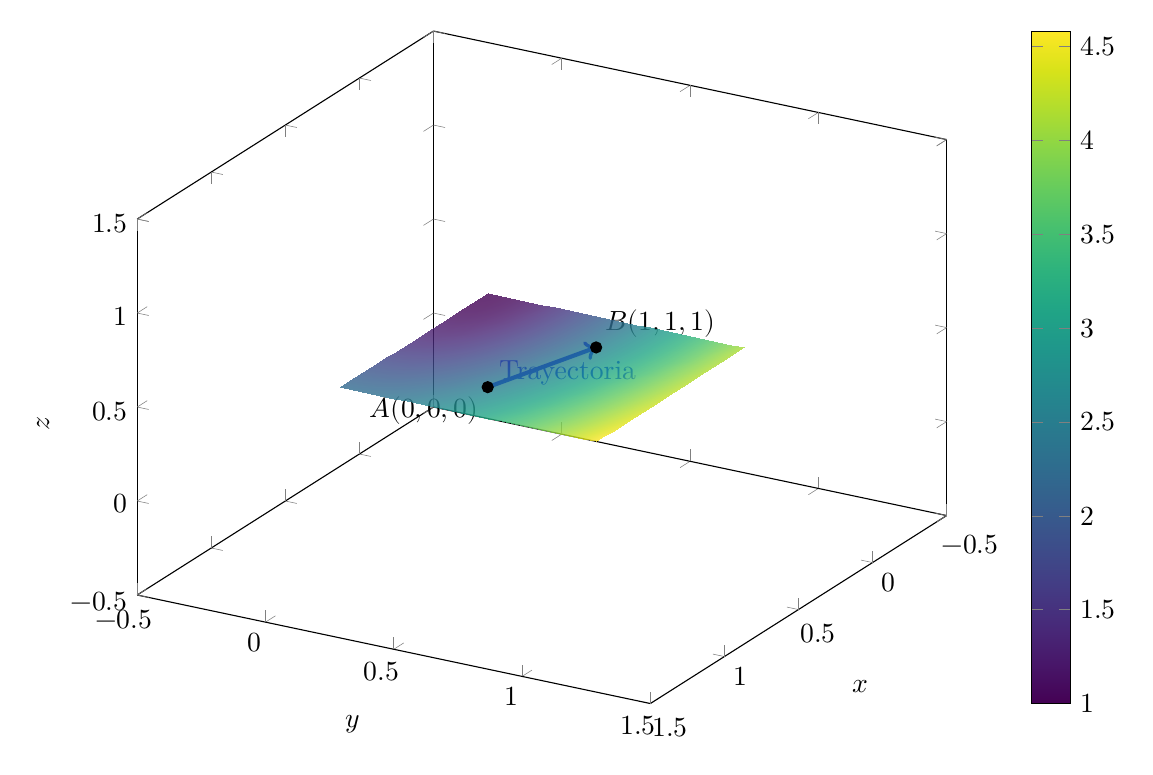
\begin{tikzpicture}
    \begin{axis}[
        scale=1.5,
        xlabel={$x$}, ylabel={$y$}, zlabel={$z$},
        xmin=-0.5, xmax=1.5,
        ymin=-0.5, ymax=1.5,
        zmin=-0.5, zmax=1.5,
        view={120}{30}, % Ajusta el ángulo de vista
        colorbar, % Muestra la barra de colores
        colormap name=viridis, % Elige el mapa de colores (puedes cambiarlo)
        point meta={sqrt((2*x)^2+(-4*y)^2+(1)^2)}, % Magnitud del campo eléctrico
    ]

    % Puntos A y B
    \addplot3[only marks, mark=*] coordinates {(0,0,0)} node[anchor=north east] {$A(0,0,0)$};
    \addplot3[only marks, mark=*] coordinates {(1,1,1)} node[anchor=south west] {$B(1,1,1)$};

    % Trayectoria (línea recta de A a B)
    \addplot3[blue, ->, line width=1.5pt] coordinates {(0,0,0) (1,1,1)};
    \node[blue] at (axis cs:0.5,0.6,0.5) {Trayectoria};

    % Superficie para el mapa de colores (plano en z=0.5)
    \addplot3[surf, shader=interp, opacity=0.8, samples=20, domain=0:1]
        ({x}, {y}, {0.5}); % z ahora es constante e igual a 0.5

    \end{axis}
\end{tikzpicture}

\end{center}

La figura anterior muestra la trayectoria de integración (línea azul) desde el punto $A$ hasta el punto $B$. Para visualizar la magnitud del campo eléctrico $\vec{E}(x, y, z) = 2x\hat{x} - 4y\hat{y} + \hat{z}$, se ha graficado un plano a una altura constante de $z=0.5$ sobre el cual se dibuja un mapa de colores.  **Este plano no representa una superficie física en el problema, sino que sirve como un lienzo para representar la variación de la magnitud del campo en función de las coordenadas $x$ e $y$**.

\textbf{¿Cómo interpretar el mapa de colores?}
\begin{itemize}
    \item \textbf{Colores:}El color en cada punto del plano representa la magnitud del campo eléctrico en ese punto. Estamos usando el mapa de colores llamado "viridis", donde los colores más cálidos (como el amarillo) corresponden a magnitudes mayores, y los colores más fríos (como el azul oscuro) corresponden a magnitudes menores. Puedes consultar la barra de colores a la derecha de la gráfica para ver la correspondencia exacta entre colores y magnitudes.
    \item \textbf{Magnitud:}La magnitud del campo eléctrico en un punto $(x, y)$ se calcula como $\sqrt{(2x)^2 + (-4y)^2 + 1^2}$.  Esto significa que la magnitud del campo es mayor cuando $x$ es grande (positivo o negativo) y cuando $y$ es grande (positivo o negativo).
\end{itemize}


\textbf{En resumen:} Aunque el campo eléctrico es un campo vectorial tridimensional, la gráfica utiliza un plano en $z=0.5$ como una superficie auxiliar para mostrar cómo varía la magnitud del campo en el espacio. El color en cada punto de este plano te da una idea de la intensidad del campo eléctrico en esa región del espacio.\\

\textbf{Ejemplo 2.3 (Campo no conservativo):}

El campo de fuerza dado es $\vec{F} = x(2x-y)\hat{x} + (x+y+z)\hat{y} + 2(2z-x)\hat{z}$ [N]. Se desea calcular el trabajo total requerido para mover un cuerpo en un círculo de radio 1 m, centrado en el origen, en el plano $x$-$y$ ($z=0$).

\textbf{Solución:}

El trabajo total realizado por el campo de fuerza $\vec{F}$ a lo largo de la trayectoria circular $C$ se calcula mediante la integral de línea cerrada:

\[
W = \oint_C \vec{F} \cdot d\vec{l}
\]

1. Parametrización de la curva en coordenadas cilíndricas:

Dado que la trayectoria es un círculo de radio 1 en el plano $x$-$y$ centrado en el origen, podemos parametrizarla en coordenadas cilíndricas como:

\[
\vec{r}(t) = \rho \cos(t) \hat{x} + \rho \sin(t) \hat{y} + z \hat{z} = \cos(t)\hat{x} + \sin(t)\hat{y}
\]

donde $\rho = 1$ (radio del círculo), $z=0$ (plano $x$-$y$), y el parámetro $t$ varía de $0$ a $2\pi$ para una vuelta completa.

2. Derivada del vector de posición:

\[
\vec{r}'(t) = \frac{d\vec{r}}{dt} = -\sin(t)\hat{x} + \cos(t)\hat{y}
\]

3. Elemento de longitud de arco en coordenadas cilíndricas:

En este caso, como estamos en el plano $x$-$y$ ($z=0$) y el radio es constante ($\rho = 1$), el elemento de longitud de arco es simplemente:

\[
d\vec{l} = \vec{r}'(t) dt = (-\sin(t)\hat{x} + \cos(t)\hat{y}) dt
\]

4. Evaluación del campo vectorial en la curva:

Primero, expresamos el campo vectorial en coordenadas cilíndricas. En general, las relaciones de transformación son:

$x = \rho \cos(t)$,
$y = \rho \sin(t)$,
$z = z$

Como estamos en el plano $x$-$y$ con radio 1, sustituimos $x = \cos(t)$, $y = \sin(t)$ y $z = 0$ en el campo $\vec{F}$:

\[
\vec{F}(\vec{r}(t)) = \cos(t)(2\cos(t)-\sin(t))\hat{x} + (\cos(t)+\sin(t))\hat{y} + 2(0-\cos(t))\hat{z}
\]
\[
\vec{F}(\vec{r}(t)) = (2\cos^2(t) - \sin(t)\cos(t))\hat{x} + (\cos(t) + \sin(t))\hat{y} - 2\cos(t)\hat{z}
\]
5. Producto punto:
\[
\vec{F}(\vec{r}(t)) \cdot d\vec{l} = [(2\cos^2(t) - \sin(t)\cos(t))(-\sin(t)) + (\cos(t) + \sin(t))(\cos(t))] \, dt
\]
\[
\vec{F}(\vec{r}(t)) \cdot d\vec{l} = [-2\cos^2(t)\sin(t) + \sin^2(t)\cos(t) + \cos^2(t) + \sin(t)\cos(t)] \, dt
\]
6. Integral de línea:
\[
W = \oint_C \vec{F} \cdot d\vec{l} = \int_0^{2\pi} [-2\cos^2(t)\sin(t) + \sin^2(t)\cos(t) + \cos^2(t) + \sin(t)\cos(t)] \, dt
\]
Resolviendo la integral (puedes usar identidades trigonométricas o un software de cálculo simbólico):
\[
\begin{aligned}
    W &= \int_0^{2\pi} [-2\cos^2(t)\sin(t) + \sin^2(t)\cos(t) + \cos^2(t) + \sin(t)\cos(t)] \, dt \\
    &= \int_0^{2\pi} -2\cos^2(t)\sin(t) \, dt + \int_0^{2\pi} \sin^2(t)\cos(t) \, dt + \int_0^{2\pi} \cos^2(t) \, dt + \int_0^{2\pi} \sin(t)\cos(t) \, dt \\
    &= \left[\frac{2}{3}\cos^3(t)\right]_0^{2\pi} + \left[\frac{1}{3}\sin^3(t)\right]_0^{2\pi} + \left[\frac{t}{2} + \frac{1}{4}\sin(2t)\right]_0^{2\pi} + \left[\frac{1}{2}\sin^2(t)\right]_0^{2\pi} \\
    &= \left(\frac{2}{3} - \frac{2}{3}\right) + (0 - 0) + \left(\frac{2\pi}{2} + 0 - 0 - 0\right) + (0 - 0) \\
    &= \pi
\end{aligned}
\]
\textbf{Resultado:}El trabajo total realizado por el campo de fuerza $\vec{F}$ para mover el cuerpo a lo largo de la trayectoria circular es $\pi$ Joules.

\textbf{Conclusión:} Como el trabajo es distinto de cero, podemos concluir que el campo de fuerza **no es conservativo**.
    \begin{center}
        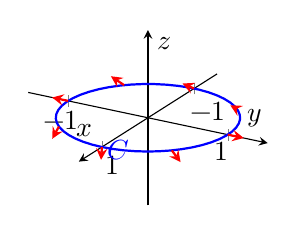
\begin{tikzpicture}
            \begin{axis}[
                scale=0.7, % Reducida la escala
                axis lines=center,
                xlabel={$x$}, ylabel={$y$}, zlabel={$z$},
                xmin=-1.5, xmax=1.5,
                ymin=-1.5, ymax=1.5,
                zmin=-1.5, zmax=1.5,
                view={120}{30},
                xtick={-1,0,1},
                ytick={-1,0,1},
                ztick={0}
            ]

            % Trayectoria circular
            \addplot3[domain=0:2*pi, samples=50, thick, blue, samples y=0] ({cos(deg(x))}, {sin(deg(x))}, {0});

            % Campo vectorial (evaluado en la trayectoria)
            \foreach \angle in {0,45,...,315} {
                \pgfmathsetmacro{\xval}{cos(\angle)};
                \pgfmathsetmacro{\yval}{sin(\angle)};
                \pgfmathsetmacro{\zval}{0};
                \pgfmathsetmacro{\uval}{\xval*(2*\xval-\yval)};
                \pgfmathsetmacro{\vval}{\xval+\yval+\zval};
                \pgfmathsetmacro{\wval}{2*(2*\zval-\xval)};
                \pgfmathsetmacro{\norm}{sqrt((\uval)^2+(\vval)^2+(\wval)^2)};
                % Dibuja la flecha solo si la norma es mayor que un valor mínimo para evitar divisiones por cero o flechas extremadamente pequeñas
                \ifdim \norm pt > 0.01pt
                    \addplot3[red, ->, >=stealth, thick] coordinates {(\xval,\yval,\zval) ({\xval+0.2*\uval/\norm},{\yval+0.2*\vval/\norm},{\zval+0.2*\wval/\norm})};
                \fi
            }
            % Ajuste de la posición de la etiqueta 'C'
            \node[blue] at (axis cs:1.1,0,0) [anchor=west] {$C$};
            \end{axis}
        \end{tikzpicture}
        \captionof{figure}{Campo de fuerza no conservativo $\vec{F}$ a lo largo de la trayectoria circular $C$ en el plano $x$-$y$.}
        \label{fig:campo_no_conservativo}
    \end{center}
    
\subsection{Integrales de Superficie}

Así como las integrales de línea generalizan la integral definida a lo largo de una curva en el espacio, las integrales de superficie extienden el concepto de integración a superficies en el espacio tridimensional. Estas integrales nos permiten calcular cantidades físicas como el flujo de un campo vectorial a través de una superficie, la masa de una superficie con densidad variable, o el área de una superficie curva.

\textbf{Definición:}

Consideremos una superficie $S$ en el espacio y un campo vectorial $\vec{A}(x,y,z)$ definido en una región que contiene a $S$. Dividamos la superficie en $n$ pequeños elementos de área $\Delta S_i$, donde $i = 1, 2, ..., n$. A cada elemento de área $\Delta S_i$ le asociamos un vector normal unitario $\hat{n}_i$, que es perpendicular a la superficie en ese punto.

La dirección del vector normal unitario depende de si la superficie es abierta o cerrada:

\begin{itemize}
    \item \textbf{Superficie cerrada:} Para una superficie cerrada, la dirección positiva del vector normal unitario es siempre la que apunta \textbf{hacia afuera} del volumen encerrado por la superficie 
    \begin{figure}[h]
    \centering
    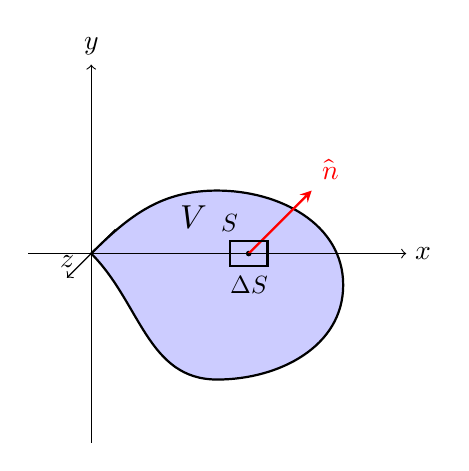
\begin{tikzpicture}[scale=0.8]
        % Dibuja la superficie cerrada (una forma irregular)
        \draw[thick, fill=blue!20] (0,0) to[out=45,in=180] (2,1) to[out=0,in=90] (4,-0.5) to[out=270,in=0] (2,-2) to[out=180,in=315] (0,0);

        % Etiqueta de la superficie
        \node at (2, 0.3,-0.5) {\small$S$};

        % Punto en la superficie
        \filldraw (2.5,0) circle (1pt);

        % Vector normal unitario
        \draw[->, >=stealth, thick, red] (2.5,0) -- (3.5,1) node[anchor=south west] {$\hat{n}$};

        % Elemento de área (pequeño rectángulo)
        \draw[thick] (2.2,-0.2) rectangle (2.8,0.2);
        \node at (2.5, -0.5) {\small$\Delta S$};
        
        % Volumen encerrado
        \node at (1.5,0.5,-0.2) {\large$V$};

        % Ejes (opcional, para dar contexto)
        \draw[->] (-1,0,0) -- (5,0,0) node[right] {$x$};
        \draw[->] (0,-3,0) -- (0,3,0) node[above] {$y$};
        \draw[->] (0,0,-1) -- (0,0,1) node[above] {$z$};
    \end{tikzpicture}
    \caption{Superficie cerrada con vector normal unitario apuntando hacia afuera.}
    \label{fig:sup_cerrada}
\end{figure}
   
    \item \textbf{Superficie abierta:} Para una superficie abierta, la dirección positiva del vector normal se define a partir del contorno que encierra la superficie. Se aplica la \textbf{regla de la mano derecha:} si los dedos de la mano derecha se curvan en la dirección de recorrido del contorno (como al evaluar una integral de línea a lo largo del contorno), el pulgar apunta en la dirección del vector normal positivo.
    \begin{figure}[h]
    \centering
    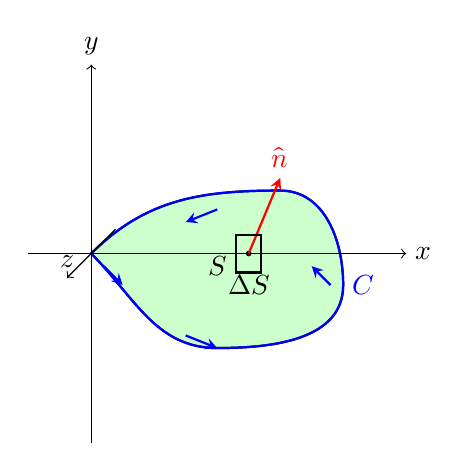
\begin{tikzpicture}[scale=0.8]
        % Dibuja la superficie abierta (una forma irregular)
        \draw[thick, fill=green!20] (0,0) to[out=45,in=180] (3,1) to[out=0,in=90] (4,-0.5) to[out=270,in=0] (2,-1.5) to[out=180,in=315] (0,0);

        % Etiqueta de la superficie
        \node at (2, -0.2) {$S$};

        % Contorno de la superficie (borde)
        \draw[thick, blue] (0,0) to[out=45,in=180] (3,1) to[out=0,in=90] (4,-0.5) to[out=270,in=0] (2,-1.5) to[out=180,in=315] (0,0);

        % Flechas a lo largo del contorno (para la regla de la mano derecha)
        \draw[<-, >=stealth, thick, blue] (1.5,0.5) -- (2,0.7); % Flecha 1 (invertida)
        \draw[<-, >=stealth, thick, blue] (3.5,-0.2) -- (3.8,-0.5); % Flecha 2 (invertida)
        \draw[<-, >=stealth, thick, blue] (2,-1.5) -- (1.5, -1.3); % Flecha 3 (invertida)
        \draw[<-, >=stealth, thick, blue] (0.5,-0.5) -- (0.2,-0.2); % Flecha 4 (invertida)

        % Etiqueta del contorno
        \node[blue] at (4, -0.5) [anchor=west] {$C$};

        % Punto en la superficie
        \filldraw (2.5,0) circle (1pt);

        % Vector normal unitario
        \draw[->, >=stealth, thick, red] (2.5,0) -- (3,1.2) node[anchor=south] {$\hat{n}$};

        % Elemento de área (pequeño rectángulo)
        \draw[thick] (2.3,-0.3) rectangle (2.7,0.3);
        \node at (2.5, -0.5) {$\Delta S$};

        % Ejes (opcional, para dar contexto)
        \draw[->] (-1,0,0) -- (5,0,0) node[right] {$x$};
        \draw[->] (0,-3,0) -- (0,3,0) node[above] {$y$};
        \draw[->] (0,0,-1) -- (0,0,1) node[above] {$z$};
    \end{tikzpicture}
    \caption{Superficie abierta con vector normal unitario definido por la regla de la mano derecha.}
    \label{fig:sup_abierta}
\end{figure}
\end{itemize}

Podemos aproximar la proyección del campo vectorial $\vec{A}$ sobre cada elemento de área $\Delta S_i$ mediante el producto escalar $\vec{A}_i \cdot \hat{n}_i \Delta S_i$, donde $\vec{A}_i$ es el valor del campo vectorial en algún punto del elemento de área $i$. Si sumamos estas proyecciones sobre toda la superficie $S$, obtenemos una aproximación de la integral de superficie de $\vec{A}$ sobre $S$:

\[
\sum_{i=1}^n \vec{A}_i \cdot \hat{n}_i \Delta S_i
\]

Para obtener la integral de superficie exacta, tomamos el límite cuando el tamaño de los elementos de área tiende a cero (es decir, cuando $n$ tiende a infinito y $\Delta S_i$ tiende a cero). En este límite, la suma se convierte en una integral, y el elemento de área $\Delta S_i$ se convierte en el diferencial de área $dS$:

\[
\iint_S \vec{A} \cdot \hat{n} \, dS = \lim_{n \to \infty, \Delta S_i \to 0} \sum_{i=1}^n \vec{A}_i \cdot \hat{n}_i \Delta S_i
\]

Esta integral también se puede escribir de forma compacta como:

\[
\iint_S \vec{A} \cdot d\vec{S}
\]

donde $d\vec{S} = \hat{n} \, dS$ es el vector diferencial de superficie, que tiene magnitud $dS$ y dirección normal a la superficie.\\

\textbf{Interpretación:} La integral de superficie de un campo vectorial $\vec{A}$ sobre una superficie $S$ representa el \textbf{flujo} del campo a través de la superficie. El producto escalar $\vec{A} \cdot \hat{n}$ nos da la componente del campo vectorial que es perpendicular a la superficie en cada punto.

\textbf{Integral de superficie de un campo escalar:}

Si en lugar de un campo vectorial tenemos un campo escalar $f(x,y,z)$, la integral de superficie se define de manera similar:

\[
\iint_S f(x, y, z) \, dS = \lim_{n \to \infty, \Delta S_i \to 0} \sum_{i=1}^n f_i \, \Delta S_i
\]

donde $f_i$ es el valor del campo escalar en algún punto del elemento de área $i$.

\textbf{Flujo a través de una superficie cerrada:}

Si la superficie $S$ es cerrada, la integral de superficie se denota con un símbolo de integral con un círculo superpuesto (similar a la circulación):

\[
\oint_S \vec{A} \cdot d\vec{S}
\]

Esta integral representa el flujo total o neto del campo vectorial $\vec{A}$ a través de la superficie cerrada $S$.

\subsubsection{Parametrización de una superficie}

Para evaluar las integrales de superficie, necesitamos una forma de describir la superficie matemáticamente. Similar a como parametrizamos una curva con un vector de posición $\vec{r}(t)$ que depende de un parámetro $t$, podemos parametrizar una superficie con un vector de posición $\vec{r}(u,v)$ que depende de dos parámetros, $u$ y $v$.

Una superficie $S$ en el espacio tridimensional se puede parametrizar mediante un vector de posición:

\[
\vec{r}(u,v) = x(u,v)\hat{x} + y(u,v)\hat{y} + z(u,v)\hat{z}
\]

donde $(u,v)$ varían en una región $D$ del plano $uv$. A medida que $(u,v)$ recorren la región $D$, el vector $\vec{r}(u,v)$ traza la superficie $S$ en el espacio.

\textbf{Analogía:} Imagine que la superficie $S$ es una sábana elástica y la región $D$ es un trozo de tela plano. La parametrización $\vec{r}(u, v)$ es como una función que nos dice cómo estirar, deformar y ubicar el trozo de tela plano $D$ en el espacio tridimensional para que coincida con la forma de la sábana $S$. Cada punto $(u, v)$ en la tela plana se mapea a un punto $(x(u,v), y(u,v), z(u,v))$ en la sábana en el espacio.
\begin{figure}[h]
    \centering
    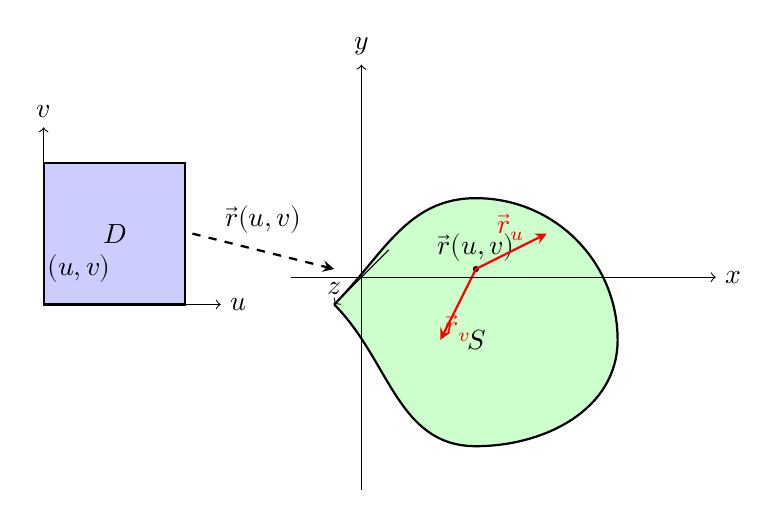
\begin{tikzpicture}[scale=0.9]
        % Plano uv (región D)
        \begin{scope}[shift={(-0.1,0)}] % Mueve el plano uv hacia la izquierda
            \draw[thick, fill=blue!20] (0,0) rectangle (2,2);
            \node at (1, 1) {$D$};
            \draw[->] (0,0) -- (2.5,0) node[right] {$u$};
            \draw[->] (0,0) -- (0,2.5) node[above] {$v$};
            \node at (0.5, 0.5) {$(u,v)$};
        \end{scope}

        % Superficie S (sábana elástica)
        \draw[thick, fill=green!20] (4,0) to[out=45,in=180] (6,1.5) to[out=0,in=90] (8,-0.5) to[out=270,in=0] (6,-2) to[out=180,in=315] (4,0);
        \node at (6, -0.5) {$S$};

        % Punto en la superficie
        \filldraw (6,0.5) circle (1pt);
        \node at (6, 0.8) {$\vec{r}(u,v)$};

        % Vectores tangentes
        \draw[->, >=stealth, thick, red] (6,0.5) -- (7,1) node[midway, above] {$\vec{r}_u$};
        \draw[->, >=stealth, thick, red] (6,0.5) -- (5.5,-0.5) node[midway, below] {$\vec{r}_v$};

        % Flecha que conecta el plano uv con la superficie
        \draw[->, >=stealth, thick, dashed] (2,1) -- (4, 0.5);
        \node at (3, 1.2) {$\vec{r}(u,v)$};

        % Ejes (opcional, para dar contexto)
        \draw[->] (3,0,-1) -- (9,0,-1) node[right] {$x$};
        \draw[->] (4,-3,-1) -- (4,3,-1) node[above] {$y$};
        \draw[->] (4,0,-2) -- (4,0,0) node[above] {$z$};

    \end{tikzpicture}
    \caption{Representación de la parametrización de una superficie $S$ mediante una región $D$ en el plano $uv$.}
    \label{fig:parametrizacion}
\end{figure}
Para calcular el elemento de área $dS$ en términos de los parámetros $u$ y $v$, necesitamos considerar cómo cambia el vector de posición $\vec{r}$ cuando variamos $u$ y $v$ ligeramente. Los vectores tangentes a la superficie en las direcciones de los parámetros $u$ y $v$ se obtienen derivando el vector de posición parcialmente con respecto a cada parámetro:

\[
\vec{r}_u = \frac{\partial \vec{r}}{\partial u} = \frac{\partial x}{\partial u}\hat{x} + \frac{\partial y}{\partial u}\hat{y} + \frac{\partial z}{\partial u}\hat{z}
\]

\[
\vec{r}_v = \frac{\partial \vec{r}}{\partial v} = \frac{\partial x}{\partial v}\hat{x} + \frac{\partial y}{\partial v}\hat{y} + \frac{\partial z}{\partial v}\hat{z}
\]

El producto cruz de estos vectores tangentes, $\vec{r}_u \times \vec{r}_v$, nos da un vector que es normal a la superficie en el punto correspondiente a los valores de $u$ y $v$. La magnitud de este producto cruz representa el factor de escala entre el área en el plano $uv$ y el área correspondiente en la superficie $S$.  \textbf{Piense en esto como el factor de "estiramiento" o "compresión" local de la tela plana al transformarla en la superficie curva.} Por lo tanto, el elemento de área $dS$ se puede expresar como:

\[
dS = |\vec{r}_u \times \vec{r}_v| \, du \, dv
\]

Y el vector diferencial de superficie $d\vec{S}$ como:

\[
d\vec{S} = \hat{n} \, dS = \frac{\vec{r}_u \times \vec{r}_v}{|\vec{r}_u \times \vec{r}_v|} \, |\vec{r}_u \times \vec{r}_v| \, du \, dv = (\vec{r}_u \times \vec{r}_v) \, du \, dv
\]

Ahora podemos expresar las integrales de superficie en términos de los parámetros $u$ y $v$:

\textbf{Para un campo vectorial} $\vec{A}(x,y,z)$:

\[
\iint_S \vec{A} \cdot d\vec{S} = \iint_S \vec{A} \cdot \hat{n} \, dS = \iint_D \vec{A}(\vec{r}(u,v)) \cdot (\vec{r}_u \times \vec{r}_v) \, du \, dv
\]

donde $\vec{A}(\vec{r}(u,v))$ significa que el campo vectorial $\vec{A}$ se evalúa en los puntos de la superficie parametrizada por $\vec{r}(u,v)$.

\textbf{Para un campo escalar} $f(x,y,z)$:

\[
\iint_S f \, dS = \iint_D f(\vec{r}(u,v)) \, |\vec{r}_u \times \vec{r}_v| \, du \, dv
\]

donde $f(\vec{r}(u,v))$ significa que el campo escalar $f$ se evalúa en los puntos de la superficie parametrizada por $\vec{r}(u,v)$.

Con estas expresiones, hemos transformado las integrales de superficie sobre la superficie $S$ en integrales dobles sobre la región $D$ del plano $uv$. Esto nos permite calcular las integrales de superficie utilizando las técnicas del cálculo de dos variables.\\

\textbf{Ejemplo 1: Integral de superficie de un campo escalar}

Enunciado: Calcule la integral de superficie del campo escalar  $$f(x, y, z) = z$$ sobre la porción del plano $x + y + z = 1$ que se encuentra en el primer octante.

\textbf{Solución:}

1. Parametrización de la superficie:

Podemos parametrizar el plano usando $x$ e $y$ como parámetros.  Despejando $z$ de la ecuación del plano, obtenemos $z = 1 - x - y$.  Entonces, la parametrización es:

\[
\vec{r}(x, y) = x\hat{x} + y\hat{y} + (1 - x - y)\hat{z}
\]

donde$(x, y)$ varían en la región triangular $D$ del plano $xy$ definida por $x \geq 0$, $y \geq 0$ y $x + y \leq 1$.

2. Vectores tangentes:

\[
\vec{r}_x = \frac{\partial \vec{r}}{\partial x} = \hat{x} - \hat{z}
\]

\[
\vec{r}_y = \frac{\partial \vec{r}}{\partial y} = \hat{y} - \hat{z}
\]

3. Producto cruz y su magnitud:

\[
\vec{r}_x \times \vec{r}_y = \begin{vmatrix}
\hat{x} & \hat{y} & \hat{z} \\
1 & 0 & -1 \\
0 & 1 & -1
\end{vmatrix} = \hat{x} + \hat{y} + \hat{z}
\]

\[
|\vec{r}_x \times \vec{r}_y| = \sqrt{1^2 + 1^2 + 1^2} = \sqrt{3}
\]

4. Evaluación del campo escalar en la superficie:

\[
f(\vec{r}(x, y)) = f(x, y, 1 - x - y) = 1 - x - y
\]

5. Integral de superficie:

\[
\iint_S f \, dS = \iint_D f(\vec{r}(x, y)) \, |\vec{r}_x \times \vec{r}_y| \, dx \, dy = \iint_D (1 - x - y) \sqrt{3} \, dx \, dy
\]

Para evaluar la integral doble, describimos la región `D` como:

$0 \leq x \leq 1$
$0 \leq y \leq 1 - x$

Entonces:

\[
\iint_S f \, dS = \sqrt{3} \int_0^1 \int_0^{1-x} (1 - x - y) \, dy \, dx = \sqrt{3} \int_0^1 \left[ y - xy - \frac{y^2}{2} \right]_0^{1-x} dx
\]

\[
= \sqrt{3} \int_0^1 \left( (1-x) - x(1-x) - \frac{(1-x)^2}{2} \right) dx = \sqrt{3} \int_0^1 \left( \frac{1}{2} - x + \frac{x^2}{2} \right) dx
\]

\[
= \sqrt{3} \left[ \frac{x}{2} - \frac{x^2}{2} + \frac{x^3}{6} \right]_0^1 = \sqrt{3} \left( \frac{1}{2} - \frac{1}{2} + \frac{1}{6} \right) = \frac{\sqrt{3}}{6}
\]

Resultado: La integral de superficie del campo escalar $f(x, y, z) = z$ sobre la porción del plano $x + y + z = 1$ en el primer octante es $\frac{\sqrt{3}}{6}$.

\begin{center}
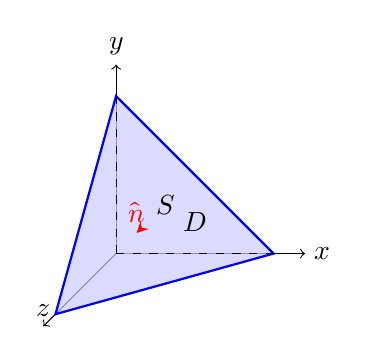
\begin{tikzpicture}[scale=2]
    % Ejes
    \draw[->] (0,0,0) -- (1.2,0,0) node[right] {$x$};
    \draw[->] (0,0,0) -- (0,1.2,0) node[above] {$y$};
    \draw[->] (0,0,0) -- (0,0,1.2) node[above] {$z$};

    % Plano
    \filldraw[fill=blue!20, opacity=0.7] (0,0,1) -- (1,0,0) -- (0,1,0) -- cycle;
    \draw[thick, blue] (0,0,1) -- (1,0,0) -- (0,1,0) -- cycle;

    % Región D en el plano xy
    \draw[dashed] (0,0,0) -- (1,0,0);
    \draw[dashed] (0,0,0) -- (0,1,0);
    \node at (0.5, 0.2, 0) {$D$};

    % Vectores normales (ejemplo)
    \draw[->, >=stealth, thick, red] (0.3,0.3,0.4) -- (0.4,0.4,0.7) node[above] {$\hat{n}$};

    % Etiquetas
    \node at (0.5, 0.5, 0.5) {$S$};

\end{tikzpicture}
\captionof{figure}{Superficie $S$ (porción del plano $x+y+z=1$ en el primer octante) y región de integración $D$ en el plano $xy$.}
\label{fig:ejemplo_sup_escalar}

\end{center}\\

\textbf{Ejemplo 2: Integral de superficie de un campo vectorial (Flujo)}

Enunciado: Calcule el flujo del campo vectorial $\vec{F}(x, y, z) = x\hat{x} + y\hat{y} + z\hat{z}$ a través de la superficie esférica $S$ de radio $R$ centrada en el origen.

\textbf{Solución:}

1. Parametrización de la superficie:

Usaremos coordenadas esféricas para parametrizar la esfera:

\[
\vec{r}(\theta, \phi) = R\sin\phi\cos\theta\hat{x} + R\sin\phi\sin\theta\hat{y} + R\cos\phi\hat{z}
\]

donde $0 \le \theta \le 2\pi$ y $0 \le \phi \le \pi$.

2. Vectores tangentes:

\[
\vec{r}_\theta = \frac{\partial \vec{r}}{\partial \theta} = -R\sin\phi\sin\theta\hat{x} + R\sin\phi\cos\theta\hat{y}
\]

\[
\vec{r}_\phi = \frac{\partial \vec{r}}{\partial \phi} = R\cos\phi\cos\theta\hat{x} + R\cos\phi\sin\theta\hat{y} - R\sin\phi\hat{z}
\]

3. Producto cruz:

\[
\vec{r}_\theta \times \vec{r}_\phi =  \begin{vmatrix}
\hat{x} & \hat{y} & \hat{z} \\
-R\sin\phi\sin\theta & R\sin\phi\cos\theta & 0 \\
R\cos\phi\cos\theta & R\cos\phi\sin\theta & -R\sin\phi
\end{vmatrix} = -R^2\sin^2\phi\cos\theta\hat{x} - R^2\sin^2\phi\sin\theta\hat{y} - R^2\sin\phi\cos\phi\hat{z}
\]

Como necesitamos que el vector normal apunte hacia afuera, tomamos el producto cruz en el orden opuesto:

\[
\vec{r}_\phi \times \vec{r}_\theta = R^2\sin^2\phi\cos\theta\hat{x} + R^2\sin^2\phi\sin\theta\hat{y} + R^2\sin\phi\cos\phi\hat{z}
\]

4. Evaluación del campo vectorial en la superficie:

\[
\vec{F}(\vec{r}(\theta, \phi)) = R\sin\phi\cos\theta\hat{x} + R\sin\phi\sin\theta\hat{y} + R\cos\phi\hat{z}
\]

5. Producto punto:

\[
\vec{F}(\vec{r}(\theta,\phi)) \cdot (\vec{r}_\phi \times \vec{r}_\theta) = R^3\sin\phi(\sin^2\phi\cos^2\theta + \sin^2\phi\sin^2\theta + \cos^2\phi) = R^3\sin\phi
\]

6. Integral de superficie:

\[
\iint_S \vec{F} \cdot d\vec{S} = \int_0^{2\pi} \int_0^{\pi} R^3\sin\phi \, d\phi \, d\theta = R^3 \int_0^{2\pi} [-\cos\phi]_0^{\pi} \, d\theta = 2R^3 \int_0^{2\pi} d\theta = 4\pi R^3
\]

Resultado: El flujo del campo vectorial $\vec{F}$ a través de la superficie esférica es $4\pi R^3$.

\begin{center}
    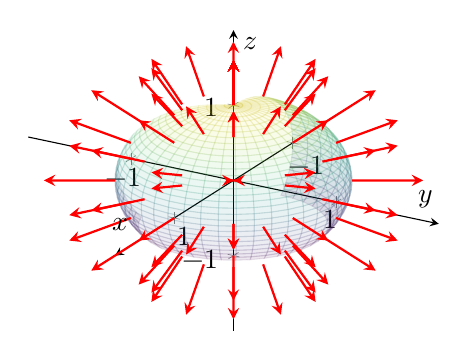
\begin{tikzpicture}
        \begin{axis}[
            scale=1.2,
            axis lines=center,
            xlabel={$x$}, ylabel={$y$}, zlabel={$z$},
            xmin=-2, xmax=2,
            ymin=-2, ymax=2,
            zmin=-2, zmax=2,
            view={120}{30},
            xtick={-1,0,1},
            ytick={-1,0,1},
            ztick={-1,0,1},
            clip=false % Permite dibujar fuera de los ejes
        ]

        % Esfera
        \addplot3[surf, domain=0:360, domain y=0:180, samples=30, opacity=0.1, colormap/viridis] ({cos(deg(x))*sin(deg(y))}, {sin(deg(x))*sin(deg(y))}, {cos(deg(y))});

        % Vectores de flujo (menos y más largos)
        \foreach \angle in {0,30,...,330} {
            \foreach \elevation in {0,30,...,150} {
                \pgfmathsetmacro{\xval}{cos(\angle)*sin(\elevation)};
                \pgfmathsetmacro{\yval}{sin(\angle)*sin(\elevation)};
                \pgfmathsetmacro{\zval}{cos(\elevation)};
                \pgfmathsetmacro{\uval}{\xval};
                \pgfmathsetmacro{\vval}{\yval};
                \pgfmathsetmacro{\wval}{\zval};
                \pgfmathsetmacro{\norm}{sqrt((\uval)^2+(\vval)^2+(\wval)^2)};
                % Dibuja la flecha solo si la norma es mayor que un valor mínimo
                \ifdim \norm pt > 0.01pt
                    \addplot3[red, ->, >=stealth, thick] coordinates {(\xval,\yval,\zval) ({\xval+0.6*\uval/\norm},{\yval+0.6*\vval/\norm},{\zval+0.6*\wval/\norm})}; % Flechas más largas
                \fi
            }
        }

        % Etiquetas de los ejes (fuera del axis environment)
       % \node[right] at (axis cs:1.5,0,0) {$x$};
       % \node[above] at (axis cs:0,1.5,0) {$y$};
       % \node[above] at (axis cs:0,0,1.5) {$z$};

        \end{axis}
    \end{tikzpicture}
    \captionof{figure}{Flujo del campo vectorial $\vec{F} = x\hat{x} + y\hat{y} + z\hat{z}$ a través de una superficie esférica.}
    \label{fig:ejemplo_sup_vectorial_mejorado}
\end{center}

\textbf{Ejemplo 3: Flujo de un campo vectorial a través de una superficie cilíndrica}

Enunciado: Considera un campo vectorial que podría representar, por ejemplo, un campo de velocidades de un fluido incompresible, dado por:

\[
\vec{A}(x,y,z) =  \frac{A_0}{x^2 + y^2}(-y\hat{x} + x\hat{y})
\]

donde $A_0$ es una constante. Determinar el flujo de este campo a través de la superficie cilíndrica definida por $x^2 + y^2 = R^2$, con $0 \le z \le L$.
\begin{center}
    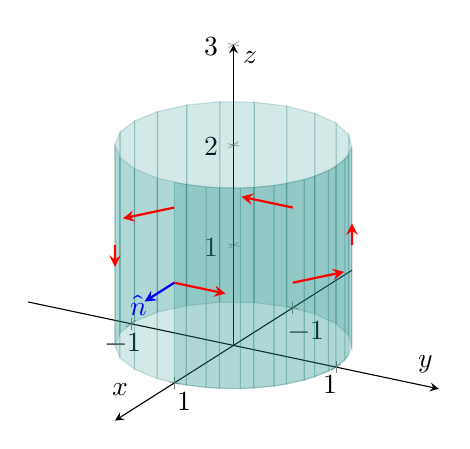
\begin{tikzpicture}
        \begin{axis}[
            scale=1.2,
            axis lines=center,
            xlabel={$x$}, ylabel={$y$}, zlabel={$z$},
            xmin=-2, xmax=2,
            ymin=-2, ymax=2,
            zmin=0, zmax=3,
            view={120}{30},
            xtick={-1,0,1},
            ytick={-1,0,1},
            ztick={0,1,2,3}
        ]

        % Cilindro
        \addplot3[surf, domain=0:360, domain y=0:2, samples=29, opacity=0.2, colormap/viridis, samples y=2] ({cos(deg(x))}, {sin(deg(x))}, {y});

        % Vectores del campo (ejemplo)
         \foreach \angle in {0,60,...,359} {
                \pgfmathsetmacro{\xval}{cos(\angle)};
                \pgfmathsetmacro{\yval}{sin(\angle)};
                \pgfmathsetmacro{\zval}{1};
                \pgfmathsetmacro{\uval}{-1*\yval};
                \pgfmathsetmacro{\vval}{\xval};
                \pgfmathsetmacro{\wval}{0};
                \addplot3[red, ->, >=stealth, thick] coordinates {(\xval,\yval,\zval) ({\xval+0.5*\uval},{\yval+0.5*\vval},{\zval+0.5*\wval})};
        }

        % Vector normal (ejemplo)
        \addplot3[blue, ->, >=stealth, thick] coordinates {(1,0,1) (1.5,0,1)};
        \node[blue] at (axis cs:1.6,0,1) {$\hat{n}$};

        \end{axis}
    \end{tikzpicture}
    \captionof{figure}{Flujo del campo $\vec{A}$ a través de una superficie cilíndrica}
    \label{fig:ejemplo_flujo_cilindro}
\end{center}

\textbf{Solución:}

El flujo del campo vectorial $\vec{A}$ a través de la superficie cilíndrica $S$ se calcula mediante la integral de superficie:

\[
\Phi = \iint_S \vec{A} \cdot d\vec{S} = \iint_S \vec{A} \cdot \hat{n} \, dS
\]

1. Parametrización de la superficie:

Usaremos coordenadas cilíndricas para parametrizar la superficie del cilindro:

\[
\vec{r}(\theta, z) = R\cos\theta\hat{x} + R\sin\theta\hat{y} + z\hat{z}
\]

donde $0 \le \theta \le 2\pi$ y $0 \le z \le L$.

2. Vectores tangentes:

\[
\vec{r}_\theta = \frac{\partial \vec{r}}{\partial \theta} = -R\sin\theta\hat{x} + R\cos\theta\hat{y}
\]

\[
\vec{r}_z = \frac{\partial \vec{r}}{\partial z} = \hat{z}
\]

3. Producto cruz y vector normal unitario:

\[
\vec{r}_\theta \times \vec{r}_z = \begin{vmatrix}
\hat{x} & \hat{y} & \hat{z} \\
-R\sin\theta & R\cos\theta & 0 \\
0 & 0 & 1
\end{vmatrix} = R\cos\theta\hat{x} + R\sin\theta\hat{y}
\]

La magnitud de este vector es:

\[
|\vec{r}_\theta \times \vec{r}_z| = \sqrt{(R\cos\theta)^2 + (R\sin\theta)^2} = R
\]

El vector normal unitario, que apunta hacia afuera de la superficie cilíndrica, es:

\[
\hat{n} = \frac{\vec{r}_\theta \times \vec{r}_z}{|\vec{r}_\theta \times \vec{r}_z|} = \cos\theta\hat{x} + \sin\theta\hat{y}
\]

4. Evaluación del campo vectorial en la superficie:

En la superficie cilíndrica, $x^2 + y^2 = R^2$. Sustituyendo en la expresión del campo vectorial:

\[
\vec{A}(\vec{r}(\theta, z)) = \frac{A_0}{R^2}(-R\sin\theta\hat{x} + R\cos\theta\hat{y}) = \frac{A_0}{R}(-\sin\theta\hat{x} + \cos\theta\hat{y})
\]

5. Producto punto:

\[
\vec{A}(\vec{r}(\theta,z)) \cdot \hat{n} = \frac{A_0}{R}(-\sin\theta\hat{x} + \cos\theta\hat{y}) \cdot (\cos\theta\hat{x} + \sin\theta\hat{y}) = \frac{A_0}{R}(-\sin\theta\cos\theta + \cos\theta\sin\theta) = 0
\]

6. Integral de superficie:

\[
\Phi = \iint_S \vec{A} \cdot \hat{n} \, dS = \int_0^L \int_0^{2\pi} \frac{A_0}{R}(-\sin\theta\hat{x} + \cos\theta\hat{y}) \cdot (\cos\theta\hat{x} + \sin\theta\hat{y}) R \, d\theta \, dz = \int_0^L \int_0^{2\pi} 0 \, d\theta \, dz = 0
\]

Resultado: El flujo del campo vectorial $\vec{A}$ a través de la superficie cilíndrica es cero.



\textbf{Conclusión:} Este resultado indica que la cantidad de "flujo" del campo vectorial $\vec{A}$ que entra a la superficie cilíndrica es igual a la cantidad que sale. Esto tiene sentido si visualizamos el campo $\vec{A}$, que representa un giro alrededor del eje $z$. La figura \ref{fig:ejemplo_flujo_cilindro} muestra una representación gráfica del campo vectorial sobre la superficie del cilindro.
    

\end{document}